\documentclass{article}
\usepackage[utf8]{inputenc}
\usepackage{tabularx,lipsum,environ,amsmath,amssymb}
\usepackage{kotex, amsthm, mathtools, enumitem, systeme, bbm, physics}

\makeatletter
\newcommand{\problemtitle}[1]{\gdef\@problemtitle{#1}}% Store problem title
\newcommand{\probleminput}[1]{\gdef\@probleminput{#1}}% Store problem input
\newcommand{\problemquestion}[1]{\gdef\@problemquestion{#1}}% Store problem question
\NewEnviron{problem}{
  \problemtitle{}\probleminput{}\problemquestion{}% Default input is empty
  \BODY% Parse input
  \par\addvspace{.5\baselineskip}
  \noindent
  \begin{tabularx}{\textwidth}{@{\hspace{\parindent}} l X c}
    \multicolumn{2}{@{\hspace{\parindent}}l}{\@problemtitle} \\% Title
    \textbf{Input:} & \@probleminput \\% Input
    \textbf{Question:} & \@problemquestion% Question
  \end{tabularx}
  \par\addvspace{.5\baselineskip}
}

\DeclareMathOperator{\AGGR}{AGGREGATE}
\DeclareMathOperator{\COMB}{COMBINE}

 
\title{EE531 Final Project Proposal}
\author{Junghyun Lee, 20170500}
\date{11/14/2019}
 
\begin{document}
 
\maketitle
 
\tableofcontents
 
\section{Fairness}
\indent
Recently, there has been an extensive study of \textit{fairness} in the context of machine learning.
As machine learning is increasingly used to make consequential classification decisions about individuals, there have been, and still is, a concern that the classifiers obtained vi ML might discriminate based on sensitive attributes.
In other words, while the learning algorithms are not inherently biased, or unfair, the algorithms may pick up and amplify already present in the training data, or 

There are many definitions of fairness, which can be classified according to their types: individual fairness, group fairness, and subgrop fairness (Mehrabi et al., 2019)
Numerous methods have been proposed to address bias and fairness. The below three papers are just few of those, each that focus on different aspect of this problem of fairness.
 
\subsection{Paper 1}
This paper is \textit{Fair Clustering Through Fairlets (F Chierichetti et al. NeurIPS 2017)}

The authors study the question of fair clustering, a common form of unsupervised learning problem, under the \textit{disparate impact} doctrine as articulated by Feldman et al. (2015).
(In other words, each protected class must have approximately equal representation in every cluster.)

In this paper, the authors show that the problem of fair clustering can be reduced to that of classical clustering.
Specifically speaking:

\begin{enumerate}
\item Define fair variants of classical clustering problems such as k-center and k-median (Section 2)
\item Define the concepts of fairlets and fairlet decompositions, which encapsulate minimal fair sets (Section 3)
\item Show that any fair clustering problem can be reduced to first finding a fairlet decomposition, and then using the classical (not necessarily fair) clustering algorithm
\item Develop approximation algorithms for finding fair decompositions for a large range of fairness values, and complement these results with NP-hardness
\item Empirically quantify the price of fairness, i.e., the ratio of the cost of traditional clustering to the cost of fair clustering.
\end{enumerate}

In summary, the authors gave efficient approximation algorithms for finding fairlet decompositions, and proved lower bounds showing that fairness can introduce a computational bottleneck.

(Please refer to the paper for the experiment design)


\subsection{Paper 2}
This paper is \textit{Empirical Risk Minimization Under Fairness Constraints (M Donini et al. NeurIPS 2018)} 

In this paper, the authors build upon the notion of \textit{Equal Opportunity (EO)}, which defines fairness as the requirement that the true positive rate of the classifier is the same across the sensitive groups.

Their main contributions are
\begin{enumerate}
\item Provide a general framework for empirical risk minimization under fairness constraints: Fair ERM (FERM)
\item Show how a linear fairness constraint arises naturally in the framework. Using that, they have developed a novel \textit{convex} learning method that is supported by consistency properties both in terms of EO and risk of the selected model, performing favorably against state-of-the-art alternatives.
\end{enumerate}

In that framework, the authors derive both risk and fairness bounds, which shows that FERM is indeed statistically consistent (in a certain sense, Section 2.2)

Also, their algorithmic observations suggest a way to implement this approach efficiently in the setting of kernel methods. This has been confirmed from their experiments, which can be found in their paper.

\subsection{Paper 3}
This paper is \textit{Fairness Through Computationally-Bounded Awareness (MP Kim et al. NeurIPS 2018)}

In this paper, the authors studied the problem of fair classification within the framework of Dwork et al. (2012)

Dwork et al. (2012) proposed a framework to resolve the conflict that the objectives of fair classification are at odds with obtaining high-utility predictions, called \textit{fairness through awareness}.
This framework takes the perspective that a fair classifier should \textit{treat similar individuals similarly}.
It was formalized by \textit{assuming} access to a task-specific similarity metric $d$ on pairs of individuals.
The proposed notion of fairness requires that if the distance between two individuals is small, then the predictions of a fair classifier cannot be very different.

The authors relaxed the condition that the metric had to be known and proposed a new theoretical framework for fair classification based on fairness through awareness-which they dubbed as \textit{fairness through computationally-bounded awareness}.

In their new framework, authors proved some theoretical results such as
\begin{enumerate}
\item This approach maintains the simplicity and flexibility of fairness through awareness, but provably only requires a small number of random samples from the underlying metric, even though we make no structural assumptions about the metric.
\item This approach is valid even when the metric is provably not learnable.
\item This approach shows how to learn a classifier that achieves optimal utility under similarity-based fairness constraints, assuming a weaker model of limited access to the metric.
\end{enumerate}

(Please refer to the paper for the experiment design.)

\section{Graph}
\indent
Graph Neural Network, denoted as GNN, was first proposed by the seminal paper \textit{The Graph Neural Network Model (Scarselli et al. IEEE 2009)} as a new framework of neural network that extends that of the RNN and Markov chains (specifically random walk model).
GNN can deal directly with graph structured information, which has since been of a significant interest in both theoretical and applicational perspective.

Before GNN, many problems, especially whose datasets were graph structured, had to be solved with existing algorithms by going through a preprocessing phase which maps the graph structured information to a simpler representation. This, obviously, led to the loss of geometric information of the dataset e.g. topological dependence of information on each node.

But as mentioned before, GNN can directly deal with those graph data, which makes it very very powerful. Many variants of it have been proposed: GCNN(Graph Convolutional Neural Network), GCN(Graph Convolutional Network, Kipf \& Welling, 2017), GraphSAGE(Hamilton et al., 2017)...etc.

GNN is based on an information diffusion mechanism, and modern GNNs follow a neighborhood aggregation strategy: we iteratively update the representation of a node by aggregating presentations of its neighbors.

Generally speaking, the $k$-th layer of a GNN is
$$a_v^{(k)} = \AGGR^{(k)} \left( \left\{ h_u^{(k - 1)} : u \in \mathcal{N}(v) \right\} \right),
\ \ h_v^{(k)} = \COMB^{(k)} \left( h_v^{(k - 1)}, a_v^{(k)} \right)$$
where $h_v^{(k)}$ is the feature vector of node $v$ at the $k$-th iteration/layer.

 
\subsection{Paper 1}
\indent
This paper is \textit{How Powerful are Graph Neural Networks? (Keyulu Xu et al. ICLR 2019)}.

\textbf{Personally, this is my number \#1 pick for the paper in the field of graph. (Yes, I am appealing for this paper. Please...)}


The authors observed that even though many variants of GNN have already been used extensively in many applications of graph representation learning, there is limited understanding of their theoretical properties and limitations.
This paper thus proposes a theoretical framework for analyzing the expressive power of GNNs to capture different graph structures.

Previous studies have shown that there is a close connection with the GNN(Graph Neural Networks) and the Weisfeiler-Lehman(WL) graph isomorphism test, and the above framework has been largely inspired by this intimate connection. (Specifically, the 1-dimensional form of the WL test is analogous to the neighbor aggregation in GNNs)

WL graph isomorphism test is a combinatorial algorithm for the \textit{Graph Isomorphism Problem}(GI), which is
\begin{problem}
  \problemtitle{\textsc{Graph Isomorphism Problem}}
  \probleminput{$G_1 = (V_1, E_1)$, $G_2 = (V_2, E_2)$, $n$(: number of steps).}
  \problemquestion{Can one determine whether $G_1$ and $G_2$ are isomorphic under $n$ steps?}
\end{problem}

This framework enables us to analyze the representational power of GNNs. In other words, how expressive different GNN variants are in learning to represent and distinguish between different graph structures: synonymous to the above GI problem!

\begin{figure}[hbt]
  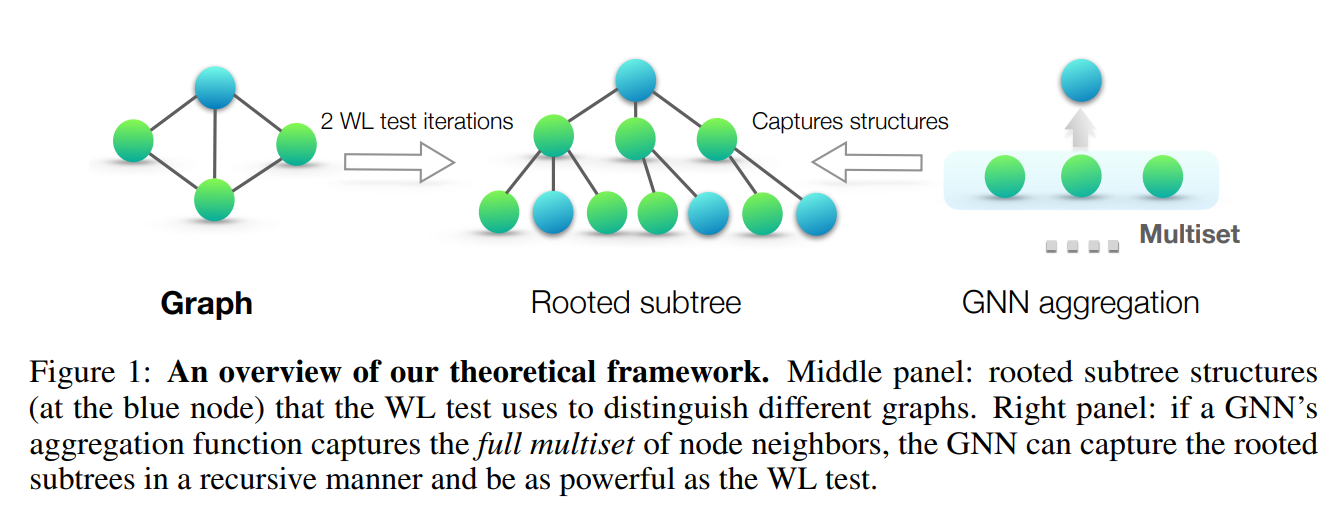
\includegraphics[height=5cm]{Figure1.png}
  \centering
\end{figure}

In summary, this paper shows the following 4 results:
\begin{enumerate}
\item GNNs are \textit{at most} as powerful as the WL test in distinguishing graph structures. (Lemma 2)
\item Under certain condition on the neighbor aggregation and graph readout functions, the resulting GNN is \textit{as powerful as} the WL test. (Theorem 3)
\item There are graph structures that cannot be distinguished by popular GNN variants, such as GCN and GraphSAGE.
\item The discriminative/representational power of \textit{Graph Isomorphism Network (GIN)}, the architecture as proposed in this paper, is equal to that of the WL test. (Section 4.1, 4.2)
\end{enumerate}

The authors evaluated and compared the training and test performance of GIN and less powerful GNN variants.
Training set performance provided a comparison between different GNN models based on their representational power, and test set performance quantifies the generalization ability.

The authors have used 9 graph classification benchmarks: 4 bioinformatics datasets (MUTAG, PTC, NCI1, PROTEINS) and 5 social network datasets (COLLAB, IMDB-BINARY, REDDIT-BINARY, REDDIT-MULTI5K).
In order ts disallow the models to rely on the input node features since the important point is for the models to learn from the network structure, authors have set the node features of the social network datasets to either be the same or one-hot encoding of node degrees.

(More specific details of the experiment design can be found in the Experiment Section of the paper)


\subsection{Paper 2}
This paper is \textit{Stochastic Training of Graph Convolutional Networks with Variance Reduction (Jianfei Chen et al., Oral, ICML 2018)}

The authors consider GCNs: a specific variant of GNN proposed by Kipf \& Welling in 2017.
GCN is a generalized version of CNN, utilizing "graph convolution" operation instead of the normal 2-D convolution.

However under the "original" GCN, the receptive field of a single node grows exponentially with respect to the number of layers, making the computation very very expensive.
Previous works to ease this include batch algorithm and neighbor sampling (NS), both of which gave a performance that is better than the original, but still expensive.

\begin{figure}[hbt]
  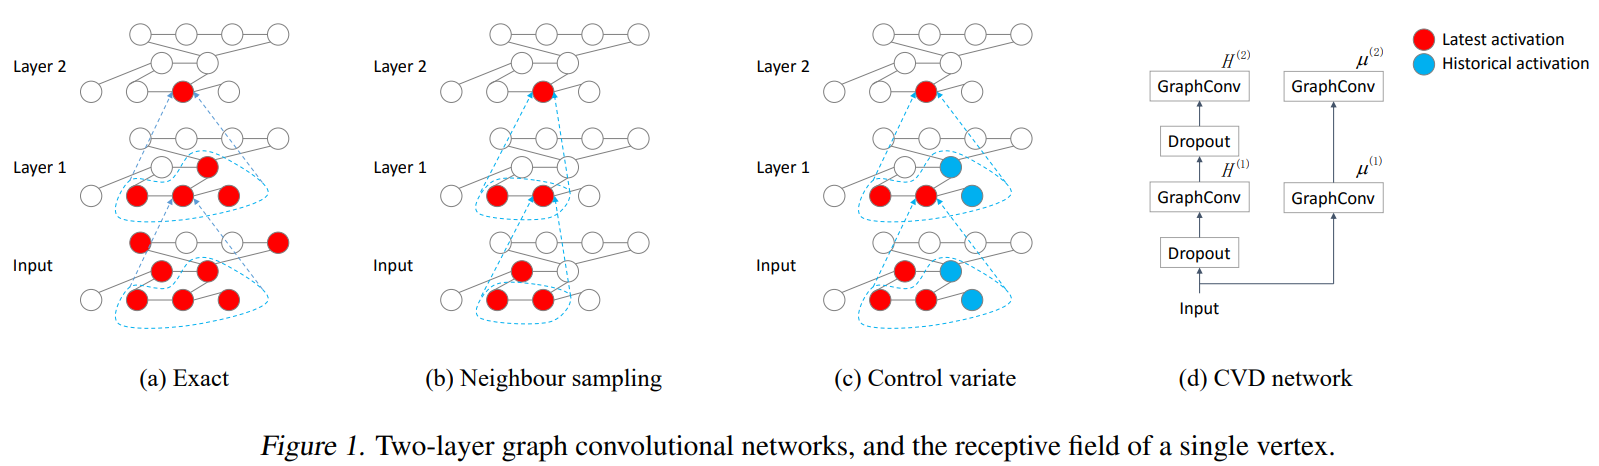
\includegraphics[width=\textwidth]{Figure2.png}
\end{figure} 

To overcome this, the authors propose a novel control variate-based stochastic approximation algorithms for GCN by utilizing the historical activation of nodes as a control variate.

(Control variates method is a variance reduction technique, mainly used in Monte Carlo methods, that exploits information abuot the errors in estimates of known quantities to reduce the error of an estimate of an unknown quantity)

Moreover, the authors show that their new algorithm has the following theoretical results:
\begin{enumerate}
\item Variance reduction from the magnitude of the activation to the magnitude of the different between current-and-historical activations
\item Exact (variance = 0) predictions at testing time
\item Convergence to a local optimum of GCN during training \textit{regardless of the neighbor sampling size $D^{(l)}$, with an asymptotically unbiased stochastic gradient.}
\end{enumerate}

Especially, the last result implies that we can obtain a significant reduction in time complexity of the stochastic training by simply choosing the sampling size as $2$, and at the same time, retain the quality of the model.

(All the above results have been also tested through experiments, as shown in the paper)


\subsection{Paper 3}
This paper is \textit{Deeper Insights into Graph Convolutional Networks for Semi-Supervised Learning (Qimai Li et al. AAAI 2019)}

Here the authors focus on the GCN and the fact that 1) its mechanisms are still unclear and 2) it still requires considerable amount of labeled data for validation and model selection.

First result is that the graph convolution of the GCN model is simply symmetric Laplacian smoothing.

Laplacian smoothing (Taubin 1995) computes the new features of a vertex as the weighted average of itself and its neighbors'.

Since vertices in the same cluster tend to be densely connected, the smoothing makes their features similar, which makes the subsequent classification task much easier.

But then, we note that an excessive application of Laplacian smoothing may mix the features of vertices from different clusters and make them indistinguishable, as shown in the diagram.

\begin{figure}[hbt]
  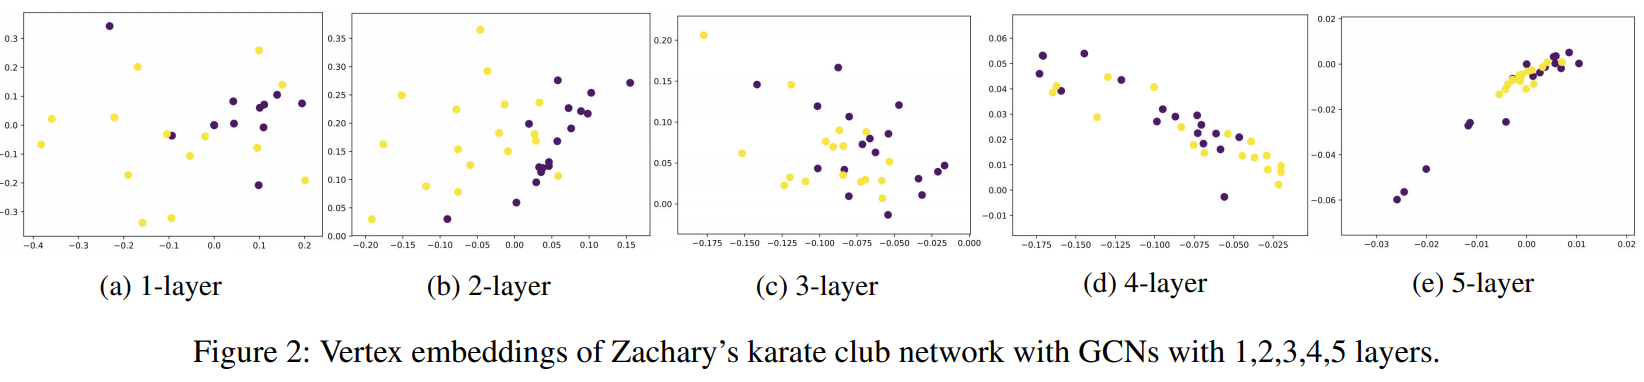
\includegraphics[width=\textwidth]{Figure3.png}
\end{figure}

Therefore we can't have many layers. But if we have too few layers, there are two problems:
1) many additional labels for validation are required
2) suffers from the localized nature of the convolutional filter

In other words, a shallow GCN cannot effectively propagate the labels to the entire data graph.
\begin{figure}[hbt]
   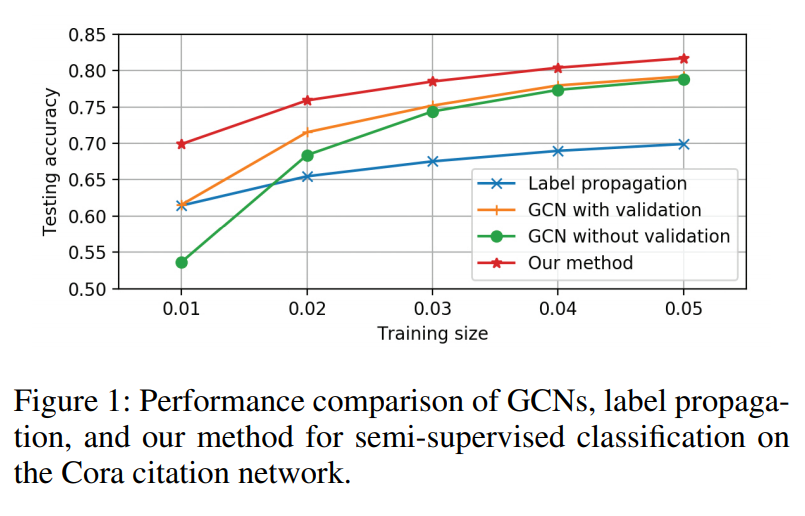
\includegraphics[height=5cm]{Figure4.png}
   \centering
\end{figure}

The authors, as a solution to this problem, proposed a approach that combines a co-training approach and a self-training approach. By co-training a GCN with a random walk model, the latter could complement the former in exploring global graph topology while by self-training a GCN, we can exploit its feature extraction capability to overcome its localized nature.

The authors also have done extensive experiments to verify their theory and the proposed methods from above. details are in the paper.

\end{document}